\documentclass[tikz,border=3pt]{standalone}
\usetikzlibrary{arrows.meta,calc}
\begin{document}
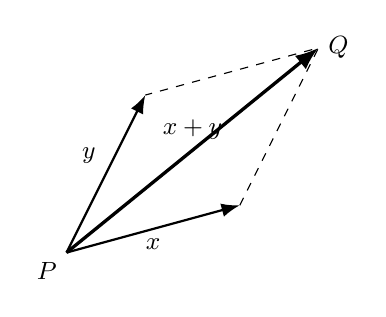
\begin{tikzpicture}[>=Latex, font=\small]
  \coordinate (P) at (0,0);
  \coordinate (X) at (2.2,0.6);
  \coordinate (Y) at (1.0,2.0);
  \coordinate (Q) at ($(X)+(Y)$);

  \draw[dashed] (X) -- (Q) -- (Y);
  \draw[->, thick] (P) -- (X) node[midway, below] {$x$};
  \draw[->, thick] (P) -- (Y) node[midway, above left] {$y$};
  \draw[->, very thick] (P) -- (Q) node[midway, above] {$x+y$};

  \node[below left] at (P) {$P$};
  \node[right] at (Q) {$Q$};
\end{tikzpicture}
\end{document}
